%%
%% getstart.tex -- Flight Gear documentation: Installation and Getting Started
%% Chapter file
%%
%% Written by Michael Basler, started September 1998.
%%
%% Copyright (C) 1999 Michael Basler (pmb@knUUt.de)
%%
%%
%% This program is free software; you can redistribute it and/or
%% modify it under the terms of the GNU General Public License as
%% published by the Free Software Foundation; either version 2 of the
%% License, or (at your option) any later version.
%%
%% This program is distributed in the hope that it will be useful, but
%% WITHOUT ANY WARRANTY; without even the implied warranty of
%% MERCHANTABILITY or FITNESS FOR A PARTICULAR PURPOSE.  See the GNU
%% General Public License for more details.
%%
%% You should have received a copy of the GNU General Public License
%% along with this program; if not, write to the Free Software
%% Foundation, Inc., 675 Mass Ave, Cambridge, MA 02139, USA.
%%
%% $Id: getstart.tex,v 0.12 1999/03/07 michael

%%%%%%%%%%%%%%%%%%%%%%%%%%%%%%%%%%%%%%%%%%%%%%%%%%%%%%%%%%%%%%%%%%%%%%%%%%%%%%%%%%%%%%%%%%%%%%%%%
\chapter{Want to have a free flight? Take {\FlightGear}!\label{free}}
%%%%%%%%%%%%%%%%%%%%%%%%%%%%%%%%%%%%%%%%%%%%%%%%%%%%%%%%%%%%%%%%%%%%%%%%%%%%%%%%%%%%%%%%%%%%%%%%%

\section{Yet another Flight Simulator?}
\markboth{\thechapter.\hspace*{1mm} WANT TO HAVE A FREE
FLIGHT?}{\thesection\hspace*{1mm} YET ANOTHER FLIGHT SIMULATOR?}

Did you ever want to fly a plane yourself, but lacked the money or
skills to do so? Do you belong to those real pilots, who want to
improve their skills without having to take off? Do you want to
try some dangerous maneuvers without risking your life? Or do you
just want to have fun with a more serious game not killing any
people? If any of these questions applies, PC flight simulators
are just for you.

If you are reading this you might have got already some experience
either using \Index{Microsoft}'s {\copyright} \Index{FS98},
\Index{Looking Glass}' {\copyright} \Index{Flight Unlimited II} or any
other of the commercially available PC flight simulators. As the price
tag of those is usually within the 50\$ range buying one of it should
not be a serious problem given the fact, that running any serious PC
flight simulator requires a hardware within the 1500\$ range, despite
dropping prices, at least.

Why then that effort of spending hundreds or thousands of hours of
programming to build a free simulator? Obviously there must be
good reason to do so:

\begin{itemize}
 \item All of the commercial programs have a serious drawback: They are made
 by a small group of developers defining their properties - often
 quite inert and not listening too much to the customer.
 Anyone ever trying to contact \Index{Microsoft} will
 immediately agree.
 \item Commercial PC flight simulators usually try to cover a market
 segment as broad as possible. For obvious reason, most of them want
 to serve the serious pilot as well as the beginner and the gamer.
 The result are compromises. As \FlightGear is free, there is no need
 for such compromises; it just can be given the properties its users
 want. It defines itself via building.
 \item Building a flight simulator is a challenge to the art of
 programming. Contributing to that project makes you belong to
 those being able to contribute to serious, ambitious and
 advanced software projects.
 \item It is fun. Not only is it fun to write the code (\ldots or
 documentation\ldots) but also to belong to that -- temporarily changing
 -- club of clever people on the net having discussed, struggled and finally
 succeeded in creating that project. Even reading the \FlightGear
 mailing lists is informative and fun for itself.
\end{itemize}

The above-mentioned points make \FlightGear different from other
competitors in several respect. \FlightGear aims to be a
civilian,\index{Flight simulator!civilian}
multi-platform,\index{Flight simulator!multi-platform}
open,\index{Flight simulator!open} user-supported,\index{Flight
simulator!user-sported} user-extensible\index{Flight
simulator!user-extensible} simulator:

\begin{itemize}
 \item \textbf{Civilian:}\index{Flight simulator!civilian} The \FlightGear
 project is primarily aimed to civilian flight simulation.
 It should be appropriate for simulating
 general aviation as well as civilian aircraft. However, according to
 the open concept of development, that sure does not exclude someone
 taking the code and integrating \Index{military components}.

 \item\textbf{Multi-platform:}\index{Flight simulator!multi-platform} The
 developers are attempting to keep the code as platform-independent
 as possible. This is based on their observation that
 people interested in flight simulations run quite
  a variety of computer hardware and operating systems. The present code
  supports the following \Index{Operating Systems}:
  \begin{itemize}
  \item\Index{Linux} (any platform),
  \item\Index{Windows NT} (i86 platform),
  \item\Index{Windows 95/98},
  \item\Index{BSD UNIX},
  \item\Index{SGI IRIX},
  \item\Index{SunOS}.
  \end{itemize}

  There is ongoing effort to support more platforms such as the
  \Index{MacIntosh}. At this time we are not aware of the existence of any other
  serious multi-platform flight simulator -- neither commercial nor free.
  Initial ideas on support for \Index{DOS} or \Index{OS/2} were dropped later because of
  diminishing interest in these platforms and the non-availability of OpenGL for DOS.

  \item\textbf{Open:}\index{Flight simulator!open} The project is not
  restricted to a closed club of developers. Anyone who feels he or she
  being able to contribute is highly welcome.
  The code (including documentation) is copyrighted under the
  terms of the \Index{Gnu Public License}.

  The Gnu Public License is often misunderstood. In simple terms it
  states that you can copy and freely distribute the program(s) licensed
  to it. You can modify them, if you like. You are even allowed to charge
  as much money for the distribution of the modified or original program as you want.
  However, you must distribute it complete with the entire source code
  and it must retain the original copyrights. In short:
\medskip

\centerline{\textit{''You can do anything with the software except
making it non-free''}.}

At present, the \Index{Gnu Public License} is not included in this
document, but can be obtained from

\web{http://www.gnu.org/copyleft/gpl.html}.

\item\textbf{User-supported, user-extensible:}\index{Flight simulator!user-supported}
  \index{Flight simulator!user-extensible}Contrary to the various
  commercial simulators available, scenery and aircraft format,
  internal variables, etc. are user accessible and documented
  from the beginning. Even without an explicit developmental \Index{documentation},
  which sure has to be written at some point, this is guaranteed by supplying the
  \Index{source code}. It is the goal of the developers to build a basic
  engine to which scenery designers, panel engineers, maybe adventure
  or ATC routine writers, sound capturers and others can (and are asked to)
  add. It is our hope, that the project will finally gain from the creativeness
  and ideas of hundreds of talented simmers across the world.

  Without doubt, the success of the \Index{Linux} project initiated by Linus
  Torvalds\index{Torvalds, Linus} inspired several of the developers.
  Not only has it shown that distributed development of even highly sophisticated
  software projects over the Internet is possible. It led to a product which,
  in several respect, is better than its commercial competitors.
\end{itemize}

\section{A short \Index{history} of \FlightGear}

This project goes back to a discussion of a group of net-citizens
in 1996. This resulted in a proposal written by David
Murr\index{Murr, David} who, unfortunately, dropped out from the
project (as well as the net) later. His \Index{proposal} is still
available from the \FlightGear web site and can be found under

\web{http://www.flightgear.org/proposal-3.0}.

Although the names of the people and several of the details
naturally changed in time, the spirit of that proposal was clearly
retained up to the present status of the project.

Actual coding started in summer 1996 and by the end of that year essential graphics
routines were completed. At that time, programming was mainly done and coordinated by
Eric Korpela\index{Korpela, Eric} from Berkeley University
(\mail{korpela@ssl.Berkeley.EDU}). Early code was running under \Index{Linux} as well as
under \Index{DOS}, \Index{OS/2}, \Index{Windows 95/NT}, and \Index{Sun-OS}. This was
quite an ambitious project, as it involved, among others, writing all the \Index{graphics
routines} in a system-independent way just from scratch.

Development slowed down and finally stopped at the beginning of 1997 when Eric had to
complete his thesis. At this point, the project seemed to be dead and traffic on the
mailing list went down to nearly nothing.

It was Curt Olson\index{Olson, Curt} from the University of Minnesota
(\mail{curt@flightgear.org}) who re-started the project in the middle of 1997. His idea
was as simple as successful: Why invent the wheel a second time? There have been several
free flight simulators\index{Flight simulator!free} available running on
\Index{workstation}s under several flavors of \Index{UNIX}. One of these,
\Index{LaRCsim}, which was developed by Bruce Jackson\index{Jackson, Bruce} from NASA
(\mail{jackson@larc.nasa.gov}) seemed to be well-adapted for the present approach. Curt
took this one apart and re-wrote several of the routines in a way making them build-able
as well as run-able on the intended target platforms. The key idea in doing so was
selecting a system-independent graphics platform, i.\,e. \Index{OpenGL}, for the basic
\Index{graphics routines}.
\medskip

 \centerline{
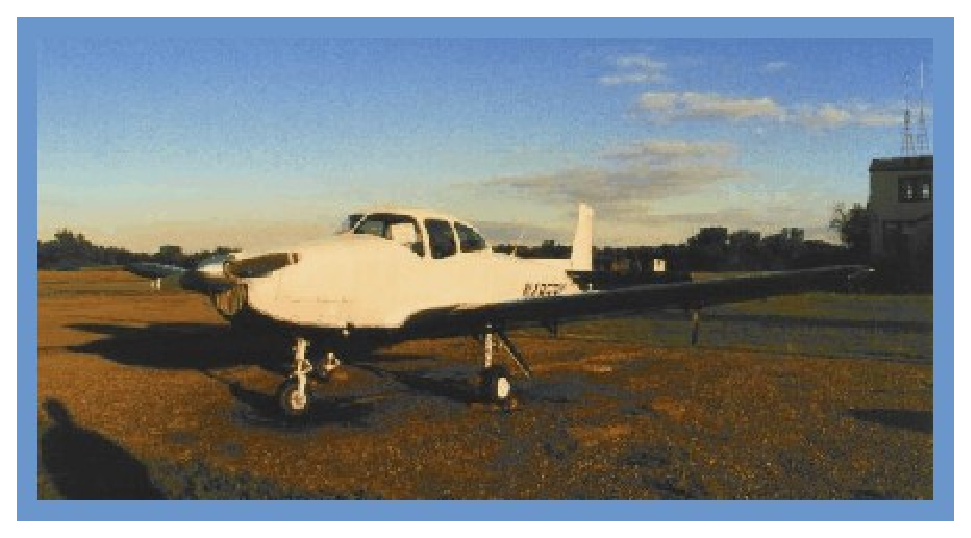
\includegraphics[clip,width=12.5cm]{navion.eps}
}

 \noindent
Fig.\,1: \textit{The \Index{Navion} flight model is one of the
features \FlightGear inherited from \Index{LaRCsim}. Until now it
is the only one plane being realized in \FlightGear.}
\medskip

In addition, a clever decision on the selection of the basic
\Index{scenery} data was already made in this very first version.
\FlightGear Scenery is created on the basis of satellite data
published by the \Index{U.\,S. Geological Survey}. These terrain
data are available for the whole world over the Internet for free
from

 \web{http://edcwww.cr.usgs.gov/doc/edchome/ndcdb/ndcdb.html}

\noindent
 for the US resp.

 \web{http://edcwww.cr.usgs.gov/landdaac/gtopo30/gtopo30.html}

\noindent
 for other countries. Those freely accessible scenery data in
 conjunction with scenery building tools provided with
 \FlightGear are an important prerequisite enabling anyone to
  create his or her own scenery, at least in principle.

This new FlightGear code - still largely being based on original \Index{LaRCsim} code -
was released in July 1997. From that moment the project gained momentum again. Here are
some milestones from the further history of development:

\begin{itemize}

\item Sun, moon and stars are a field where PC flight simulators
 have been notoriously weak for ages. It is one of the great
 achievements of \FlightGear that it includes accurate sun (watch, Microsoft!),
 moon, and planets being moreover placed on their proper positions.
 The corresponding \Index{astronomy code} was implemented in fall 1997 by Durk
 Talsma\index{Talsma, Durk}
 (\href{mailto:pn_talsma@macmail.psy.uva.nl}{pn\_talsma@macmail.psy.uva.nl}.

\item Texture support\index{textures} was added by Curt
Olson\index{Olson, Curt}
 (\mail{curt@flightgear.org}) in spring 1998. This marked a
 significant improvement in terms of reality. You may recall: MSFS had
 untextured scenery up to version 4.0. For this purpose, some high-quality
 textures were submitted by Eric Mitchell\index{Mitchell, Eric}
 (\href{mailto:mitchell@mars.ark.com}{mitchell@mars. ark.com}.

\item A \Index{HUD} (\Index{head up display}) was added based on code
 provided by Michele America\index{America, Michele} (\mail{nomimarketing@mail.telepac.pt})
and Charlie Hotch\-kiss\index{Hotchkiss, Charlie}
(\href{mailto:chotchkiss@namg.us.anritsu.com}{chotch kiss@namg.us.anritsu.com})
 in fall 1997 and continuously improved later.
 While being probably not a substitute for a \Index{panel} and moreover
 possibly being a bit odd in that tiny \Index{Navion}, this \Index{HUD} has proven
 extremely useful in navigation until now.

\item After improving scenery\index{scenery} and
texture\index{textures} support and adding some more
 features there was a disappointing side-effect in spring 1998: Frame
 rates\index{frame rate} dropped down to a point where \FlightGear became inflyable. There
 were two main achievements overcoming this problem. First, with the advent
 of hardware \Index{OpenGL} support and corresponding drivers for most of
 the graphics cards these features could be exploited in
 \FlightGear as well, leading to a \Index{frame rate} boost by a
 factor up to 10. Second, Curt Olson\index{Olson, Curt} (\mail{curt@flightgear.org})
 implemented so-called \Index{view frustrum culling} (a procedure to except part of
 the scenery not required from  rendering) which gave another 20\% or so of
 frame rate boost in May 1998.

 With these two achievements \FlightGear became flyable again even on weaker
 machines as long as they included a 3D graphics board with
 hardware \Index{OpenGL} support. (With respect to this point one should keep in mind that the code
 at present is in no way optimized leaving a lot of room for further
 improvements of frame rate.)

\item A rudimentary \Index{autopilot} implementing heading hold was
contributed by Jeff Goeke-Smith\index{Goeke-Smith, Jeff} (\mail{jgoeke@voyager.net}) in
April 1998. This autopilot was improved to cover altitude hold and a terrain follow
switch in October 1998.

\item Although detailed menus are still missing there is a first
 approach on developing a \Index{menu system} based on Steve Baker's\index{Baker, Steve}
  (\mail{sjbaker@hti.com}) menu library \Index{PUI}. This first menu
  system was added in June 1998.

\item Friedemann Reinhard \index{Reinhard, Friedemann}
(\mail{mpt218@faupt212.physik.uni-erlangen.de})
 developed early \Index{panel code} including a working \Index{airspeed
 indicator} which was added in June 1998 and has been considerably improved until today.

\item There was basic \Index{audio support}
i.\,e. an audio library and some basic background engine sound,
contributed by Steve Baker (\mail{sjbaker@hti.com})\index{Baker,
Steve} and Tom Knienieder\index{Knienieder, Tom}
(\mail{knienieder@ms.netwing.at}) in Summer 1998.

\item Steve Baker\index{Baker, Steve}
(\mail{sjbaker@hti.com}) and Curt Olson\index{Olson, Curt} (\mail{curt@flightgear.org})
got basic joystick/yoke support running in October 1998. While implementation may change
and pedals do not yet work under Windows this marks a huge improvement in terms of
realism.

\item In September 1998 Curt Olson\index{Olson, Curt}
(\mail{curt@flightgear.org}) succeeded in creating complete terrain Scenery for the USA,
which is available for download from

\web{ftp://ftp.kingmont.com/pub/kingmont/}.

\end{itemize}

\longpage

This is by no way a complete history and a lot of people making even important
contributions were left out here. Besides the named achievements which are more on the
surface, there was a lot of work done concerning the internal structure, by Steve
Baker\index{Baker, Steve} (\mail{sjbaker@hti.com})\index{Baker, Steve}, Norman
Vine\index{Vine, Norman} (\mail{nhv@laserplot.com}), Gary R. Van Sickle\index{Van Sickle,
Gary, R.} (\mail{tiberius@braemarinc.com}), and others. A more complete list of
contributors to the project can be found in \textit{Landing: Some further thoughts before
leaving the plane}, chapter \ref{landing} as well as in the file \texttt{Thanks} provided
with the code. Moreover, the \Index{\FlightGear Website} contains a detailed history of
all of the development under

\web{http://www.flightgear.org/News/}.

\section{System requirements}\index{system requirements}
Compared to other recent flight simulators the system requirements
for \FlightGear are rather decent. A P100 is already sufficient,
given you have a proper 3D graphics card, but of course for
getting good performance we recommend a P200 or better, if you run
it on a PC. On the other hand, any not too ancient \Index{UNIX}
\Index{workstation} will run \FlightGear as well.

While in principle you can run \FlightGear on 3D boards without OpenGL support or even on
systems without 3D graphics hardware, missing hardware OpenGL support can force even the
fastest PII to its knees (\Index{frame rate}s typically below 1 fps even on fast
machines). Any cheap 3D graphics card will do as long as it features hardware
\Index{OpenGL} support. For \Index{Windows 98/NT} drivers, you may contact the home page
of the manufacturer. Moreover, you should have in mind that most OpenGL
drivers\index{OpenGL!drivers} are still marked as beta and moreover, often these drivers
are provided by the makers of the graphics chip instead of the makers of the board. More
detail on OpenGL drivers can be found under

\web{http://www.x-plane.com/v4ibm.html}

\noindent
  as well as under

\web{http://www.flightgear.org/Hardware}.

Moreover, you need around 16MB of free disk space for installing the
executable including most of the scenery. In case you want to compile
the program yourself you need around 50MB for the source code and for
temporary files created during compilation, independent of the
operating system.

If you want to hear the \Index{sound effects} any decent \Index{sound card} should serve.
At present, support for using a \Index{joystick} or \Index{yoke} is just in its early
stages, but is expected to work on most systems. At present, Pedals are supported under
UNIX/Linux only.

With respect to operating systems, \FlightGear is being primarily developed under
\Index{Linux}, a free UNIX clone developed cooperatively over the net in much the same
way as the \FlightGear project itself. Moreover, \FlightGear runs under \Index{Windows
95}, \Index{Windows 98} and \Index{Windows NT} and given you have a proper
\Index{compiler} installed it can be build under all of these platform as well. The
primary compiler for all platforms is \Index{GNU C++} (i.\,e. the \Index{Cygnus} compiler
under Win32), however there is some support for \Index{MSVC}5 as well. Moreover,
\FlightGear runs and can be build on several \Index{UNIX}/X11 platforms with GNU C++
installed.

\section{Whom this guide is addressed to and how it is organized}

At first: There is not much of the material in this Guide being originally invented by
ourself. You could even say with Montaigne that we ''merely gathered here a big bunch of
other men's flowers, having furnished nothing of my own but the strip to hold them
together''. Most (but fortunately not all) of the information can as well be grabbed from
the \Index{\FlightGear home page} being situated at

\web{http://www.flightgear.org/}

 \noindent
 and its various sub pages. However, there still seem to
be a small group of people preferring neatly printed manuals over
loosely scattered Readmes and those may acknowledge our effort.

This \textit{Installation and Getting Started} is intended as being a first step towards
a more complete \Index{\FlightGear documentation} (with the other parts, supposedly, to
be written by others). Its main addressee is the end-user who is not interested in the
internal workings of \Index{OpenGL} or in building his or her own scenery, for instance.
It is our hope, that sometime there will be an accompanying \textit{\Index{\FlightGear
Programmer's Guide}}, which could be based on some of the documentation under

\web{http://www.flightgear.org/Docs},

 \noindent
a \textit{\Index{\FlightGear Scenery Design Guide}}, and a
\textit{\Index{\FlightGear Flight School}}, at least.

This \textit{Installation and Getting Started} is organized as
follows:

The first chapter \ref{opengl}, \textit{Getting the engine: Installing OpenGL graphics
drivers}, describes how to prepare the computer for handling \FlightGear's graphics
routines. \FlightGear is based on a graphics library called OpenGL, thus you must install
either hardware or software OpenGL support for your graphics board (except, you did so
before, of course).

Chapter \ref{building}, \textit{Building the plane: Compiling the program}, explains how
to build, i.\,e. compile the simulator. Depending on your platform this may or may not be
required for you. There will at least be binaries available for those working on a Win32
(i.\,e. Windows 98 {\copyright} or Windows NT {\copyright}) platform. For those on such
systems, who want to take off immediately without going through the potentially
troublesome process of compiling, we recommend just skipping that chapter and going
directly to the next one.

In chapter \ref{prefligh}, \textit{Preflight: Installing \FlightGear}, you find
instructions for installing the binaries in case you did not so by building them in the
previous chapter. Moreover, you'll have to install scenery and texture files, which will
be described there, too.

The following chapter \ref{takeoff}, \textit{Takeoff: How to start the program},
describes how to start the program including an overview on the command line options.

\textit{Flight: Keystrokes, HUD, and all that}, chapter \ref{flight}, describes how to
operate the program, i.\,e. to actually fly with \FlightGear. This includes several lists
of key strokes as well as a detailed description of the HUD (head up display) as the
primary instrument for controlling the plane.

In chapter \ref{landing}, \textit{Landing: Some further thoughts before leaving the
plane}, we would like to give credits to those who did the hard work and give an outlook
on what remains to be done.

Finally: \textbf{We kindly ask others to help us improving this document by submitting
corrections, improvements, and more. Notably, we invite others to contribute descriptions
referring to alternative setups (graphics cards, operating systems, and compilers etc.).
We will be more than happy to include those into forthcoming versions of this
\textit{Installation and Getting Started} (of course not without giving credit to the
authors).}

We hope to continuously maintain this document at least for a foreseeable future, but
probably will not be able to produce a new one for any single release of {\FlightGear}.
While we are both watching the mailing lists, it might help, if developers adding new
functionality could send us a short note.


%% Revision 0.00  1998/09/08  michael
%% Initial revision for version 0.53.
%% Revision 0.01  1998/09/20  michael
%% several extensions and corrections
%% revision 0.10  1998/10/01  michael
%% final proofreading for release
%% revision 0.11  1998/11/01  michael
%% minor corrections on platforms, satellite data, OpenGL (S. Baker)
%% added Navion pic
%% revision 0.12  1999/03/07  michael
%% update on recent development
